\section{The Case for Human-AI Trust}
    Many would not be surprised to know that trust is critical in interpersonal relationships, and that it affects the dynamics of systems as simple as interpersonal relationships to more complicated ones such as financial markets \cite{Fukuyama1995-un} and governments. Consequently, researchers in psychology, sociology, and economics have historically sought to understand the fundamental principles of trust, each with the aim of understanding their field better \cite{Gambetta1988-pi}. Moral philosophers have also thought intently about the topic \cite{Baier1986-im}.

    In the early days of the internet there was a surge of interest in trust due to the appearance of e-commerce. Suddenly, a new forum for buying and selling wares and services appeared. How could relationships of trust be built between consumers and vendors in a new `online' ecosystem? Many researchers focused their efforts on exploring how to establish an ecosystem that would nurture the growth and prosperity of online businesses \cite{McKnight2001-fa}. This research is useful to those seeking to understand trust today because it focused on building such an ecosystem. Consequently the more practical understanding emerged that included some thoughts about how to affect trust. This survey will not exhaustively review the literature on trust; those interested might refer to the following works by \citet{McKnight2001-fa}, and \citet{Lewicki2006-hj}.

    Due to wide interest spanning many disciplines it is difficult, if not impossible, to write a succinct definition that would appease all interested parties. In their work relating to e-commerce \citet{McKnight2001-fa} reviewed much of the existing trust literature and attempted to distill the main concepts into a trust model that spanned disciplines. That model is shown, with some minor adaptations, in Figure \ref{fig:UserTrust}. Notice that the three main dimensions --- Dispositional Trust, Institutional Trust, and Interpersonal Trust --- are connected in such a way as to indicate some causal relationships between them. As trust cannot be directly measured there is no existing method with which to quantify the more detailed relationships between each of the dimensions of trust.

	\begin{figure}[htbp]
    	\centering
     	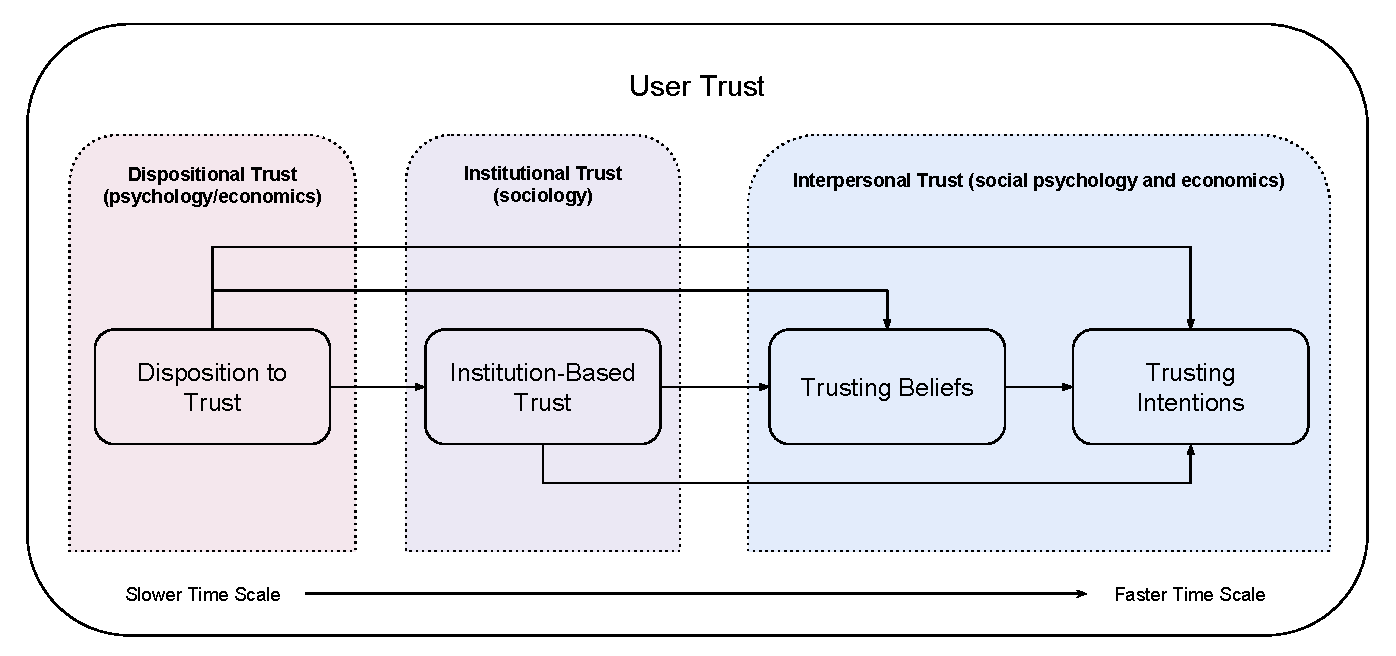
\includegraphics[width=0.9\textwidth]{Figures/UserTrust}
    	\caption{Interdisciplinary trust model proposed by \citet{McKnight2001-fa}. The three main categories are delineated and corresponding disciplines that are interested are listed within parentheses.}
        \label{fig:UserTrust}
    \end{figure}

    Something that is well accepted among researchers of all discplines is that trust results in some kind of behavior or action, which \citet{McKnight2001-fa} calls `trust-related behaviors' (TRBs). In the case of a human-autonomy relationship examples of TRBs might be the kinds of tasks the human user assigns to the autonomy, or whether the human will use a plan produced by the autonomy.


